Im Jahr 2009 veröffentlichte Ryan Dahl das Framework Node.js, das auf Googles V8-Engine, welche auch als JavaScript-Engine in Googles Browser Chrome zum Einsatz kommt, basiert und sich hervorragend für hochperformante, skalierbare und schnelle Webanwendungen eignet. Zudem ermöglicht es Webentwicklern die Entwicklung von serverseitigem JavaScript-Code. \-[NodeJS 1.0]


\subsubsection{Architektur TODO Aufzählung}
Eine wesentliche Eigenschaft von Node.js ist die hohe Performance. Im Folgenden soll der Unterschied der Node.js-Architektur zu traditionellen Webservern und der damit verbundenen höheren Performance dargestellt werden.
\newline

Herkömmliche Webserver erstellten zunächst für jede ankommende Anfrage einen neuen Thread. Dieses Vorgehen ist eng mit steigendem Speicher- und Rechenaufwand verbunden. Um sich Rechenzeit, die durch die Erstellung und Zerstörung von Threads entstanden, zu sparen, wurden Threadpools eingerichtet. Dieser Threadpool enthält mehrere Threads, denen Aufgaben zugewiesen werden können. Nach erfolgreicher Abarbeitung einer Operation kann einem Thread eine weitere Aufgabe zugeordnet werden.
\newline

Es bleibt aber ein weiteres Problem: Bei der Anfragenabarbeitung kann es zu einer Form von blockierender Ein- und Ausgabe (Blocking Input/Output kurz Blocking I/O) kommen: zum Beispiel beim Suchen in einer Datenbank oder dem Laden einer Datei im Dateisystem. Während der Abarbeitung wartet der Thread solange, bis die Operation ein Ergebnis zurückwirft und belegt dabei weiterhin Speicherplatz. Bei hohem Anfragen-aufkommen kommt es dadurch zu einer hohen Speicherauslastung des Servers. Zudem kosten die Kontextwechsel zwischen den Threads im Betriebssystem weitere Rechenzeit. [Node.js 1.05] Man spricht bei diesem Architekturkonzept auch vom Multi-Threaded Server.
\newline

\begin{figure}[h]
\centering
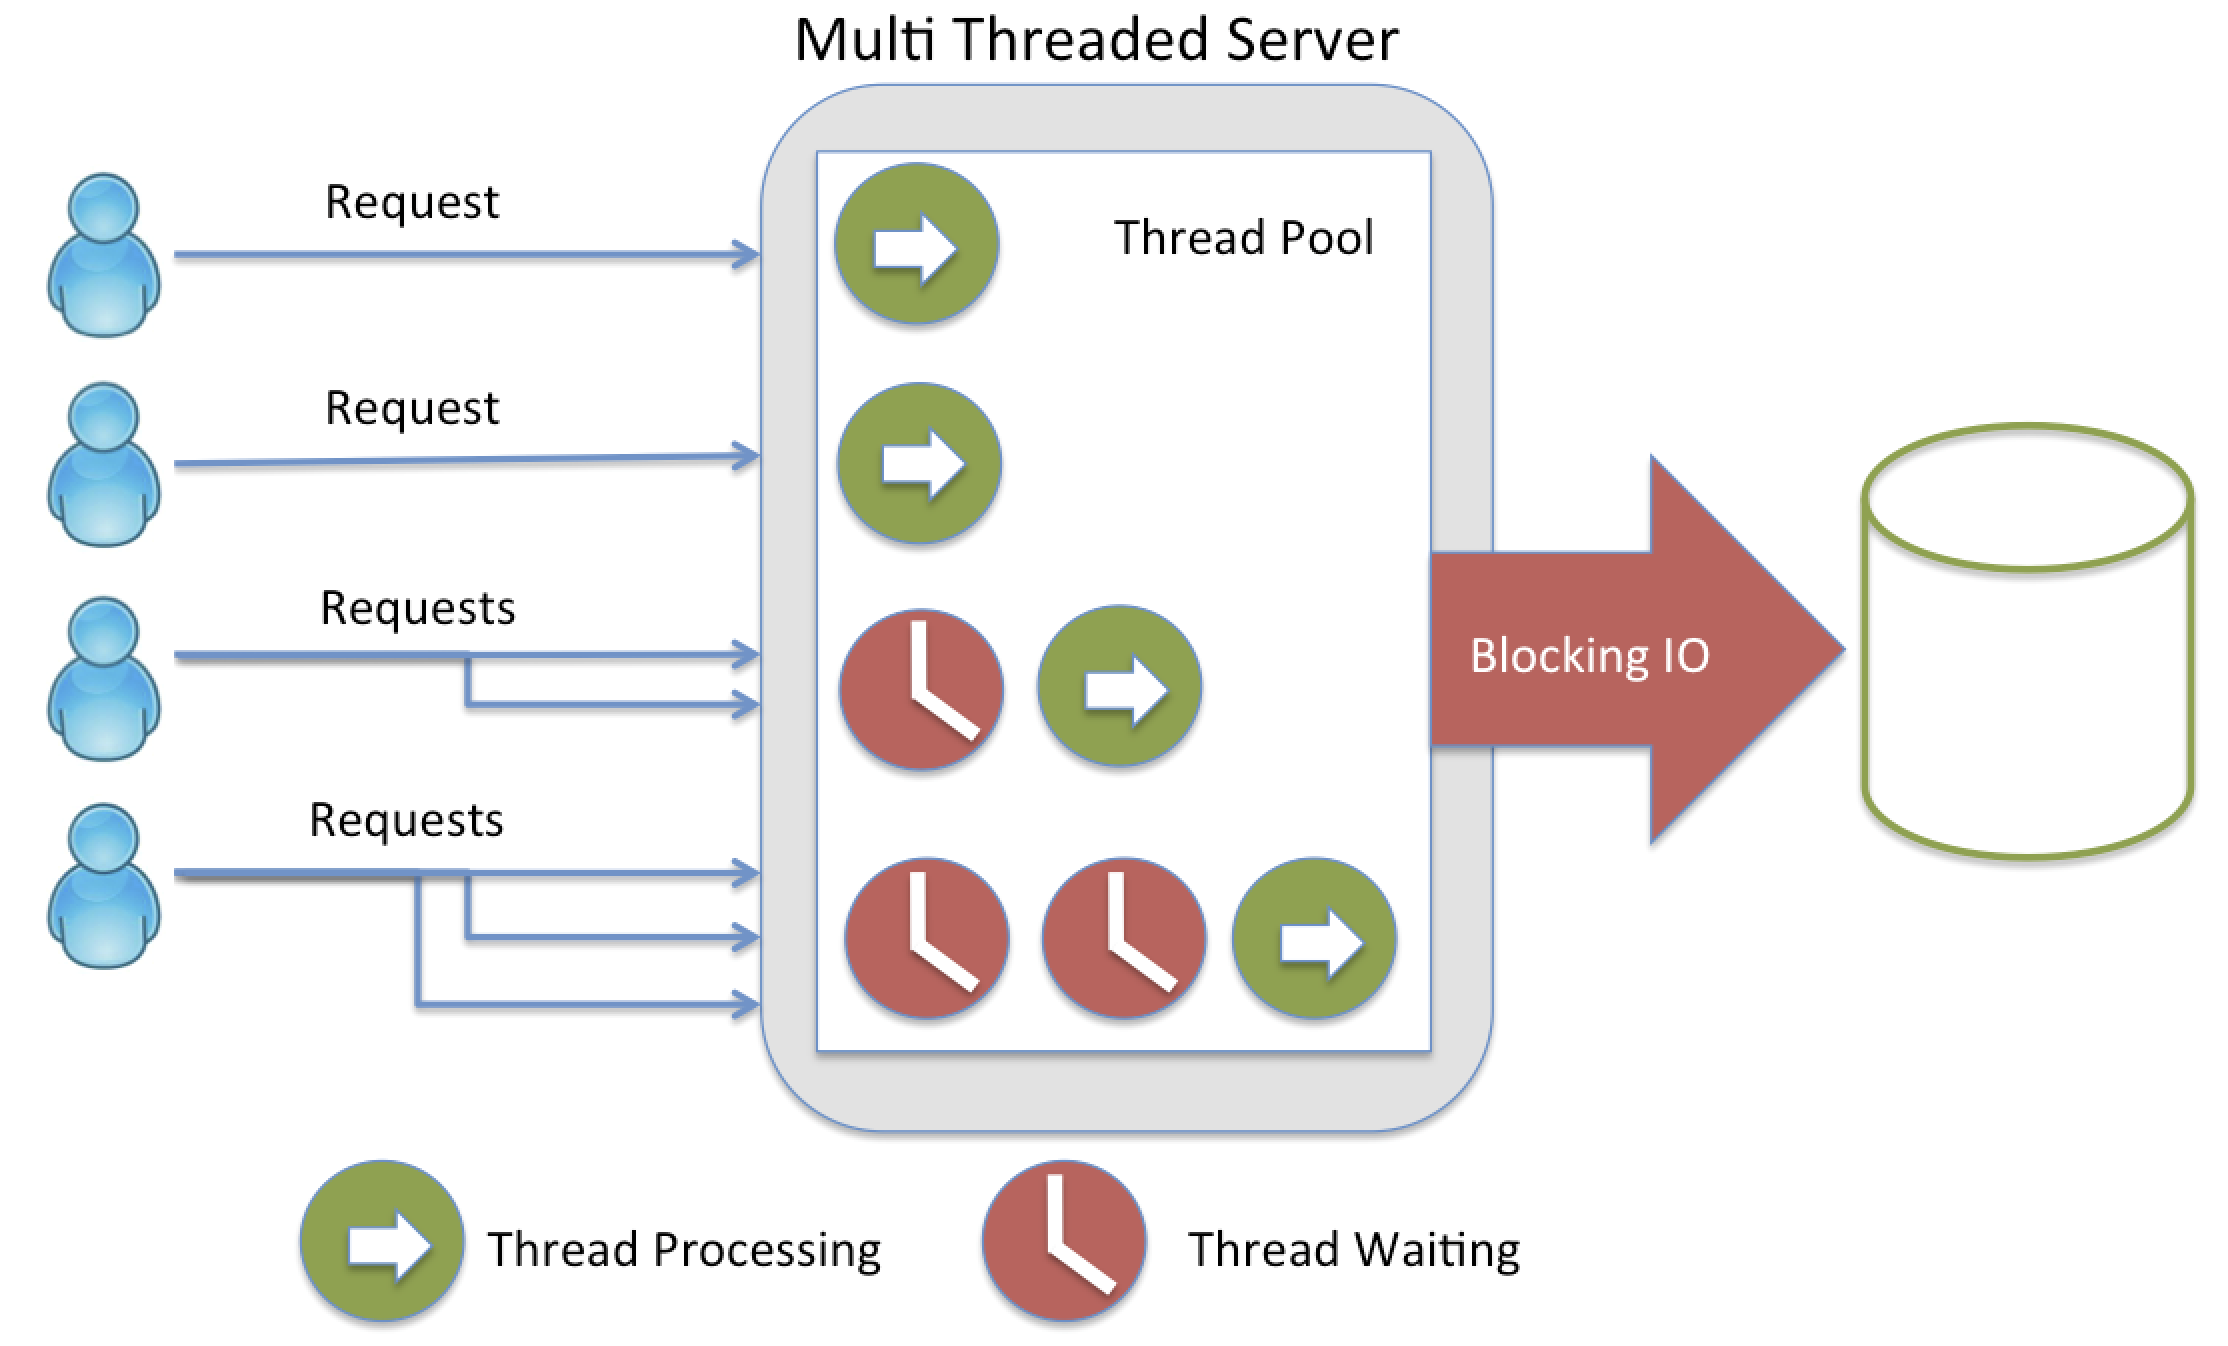
\includegraphics[width=10cm, height = 5.5cm]{images/nodejs_otherthreading.png}
\caption{Multithreaded / Blocking I/O [Nodejs 1.1]}
\end{figure}
 
\newpage

Node.js verfolgt einen anderen Ansatz: Anfragen werden nur in einem einzigen Thread, dem Hauptthread, abgearbeitet und in einer Warteschlange verwaltet. Dadurch bleiben Kontextwechsel zwischen Threads erspart. Hierbei handelt es sich also um einen Single-Threaded Server. Der Hauptthread verwaltet eine Schleife, die sogenannte Event Loop, die permanent Anfragen aus der Event-Warteschlange überprüft und Ereignisse, die von Ein- und Ausgangsoperationen ausgerufen werden, verarbeitet.
\newline

Bei Ankommen einer Nutzeranfrage an einen Node.js Server wird zunächst in der Event Loop geprüft, ob diese Anfrage Blocking I/O benötigt. Falls nicht, kann die Anfrage direkt bearbeitet werden und die Antwort an den Nutzer zurückgesendet werden. 
\newline

Im anderen Fall wird einer von Node.js interner Workern, welche prinzipiell auch Threads sind, aufgerufen, um die jeweilige Operation auszuführen. Dabei wird eine Callback-Funktion mitgegeben, die vom Worker aufgerufen wird, sobald die Operation ausgeführt wurde. Diese Callback-Funktion ist kann anschließend als Ereignis von der Event Loop registriert werden. Man spricht hierbei auch von ereignisgesteuerter Architektur. [1.4]
\newline
 
\begin{figure}[h]
\centering
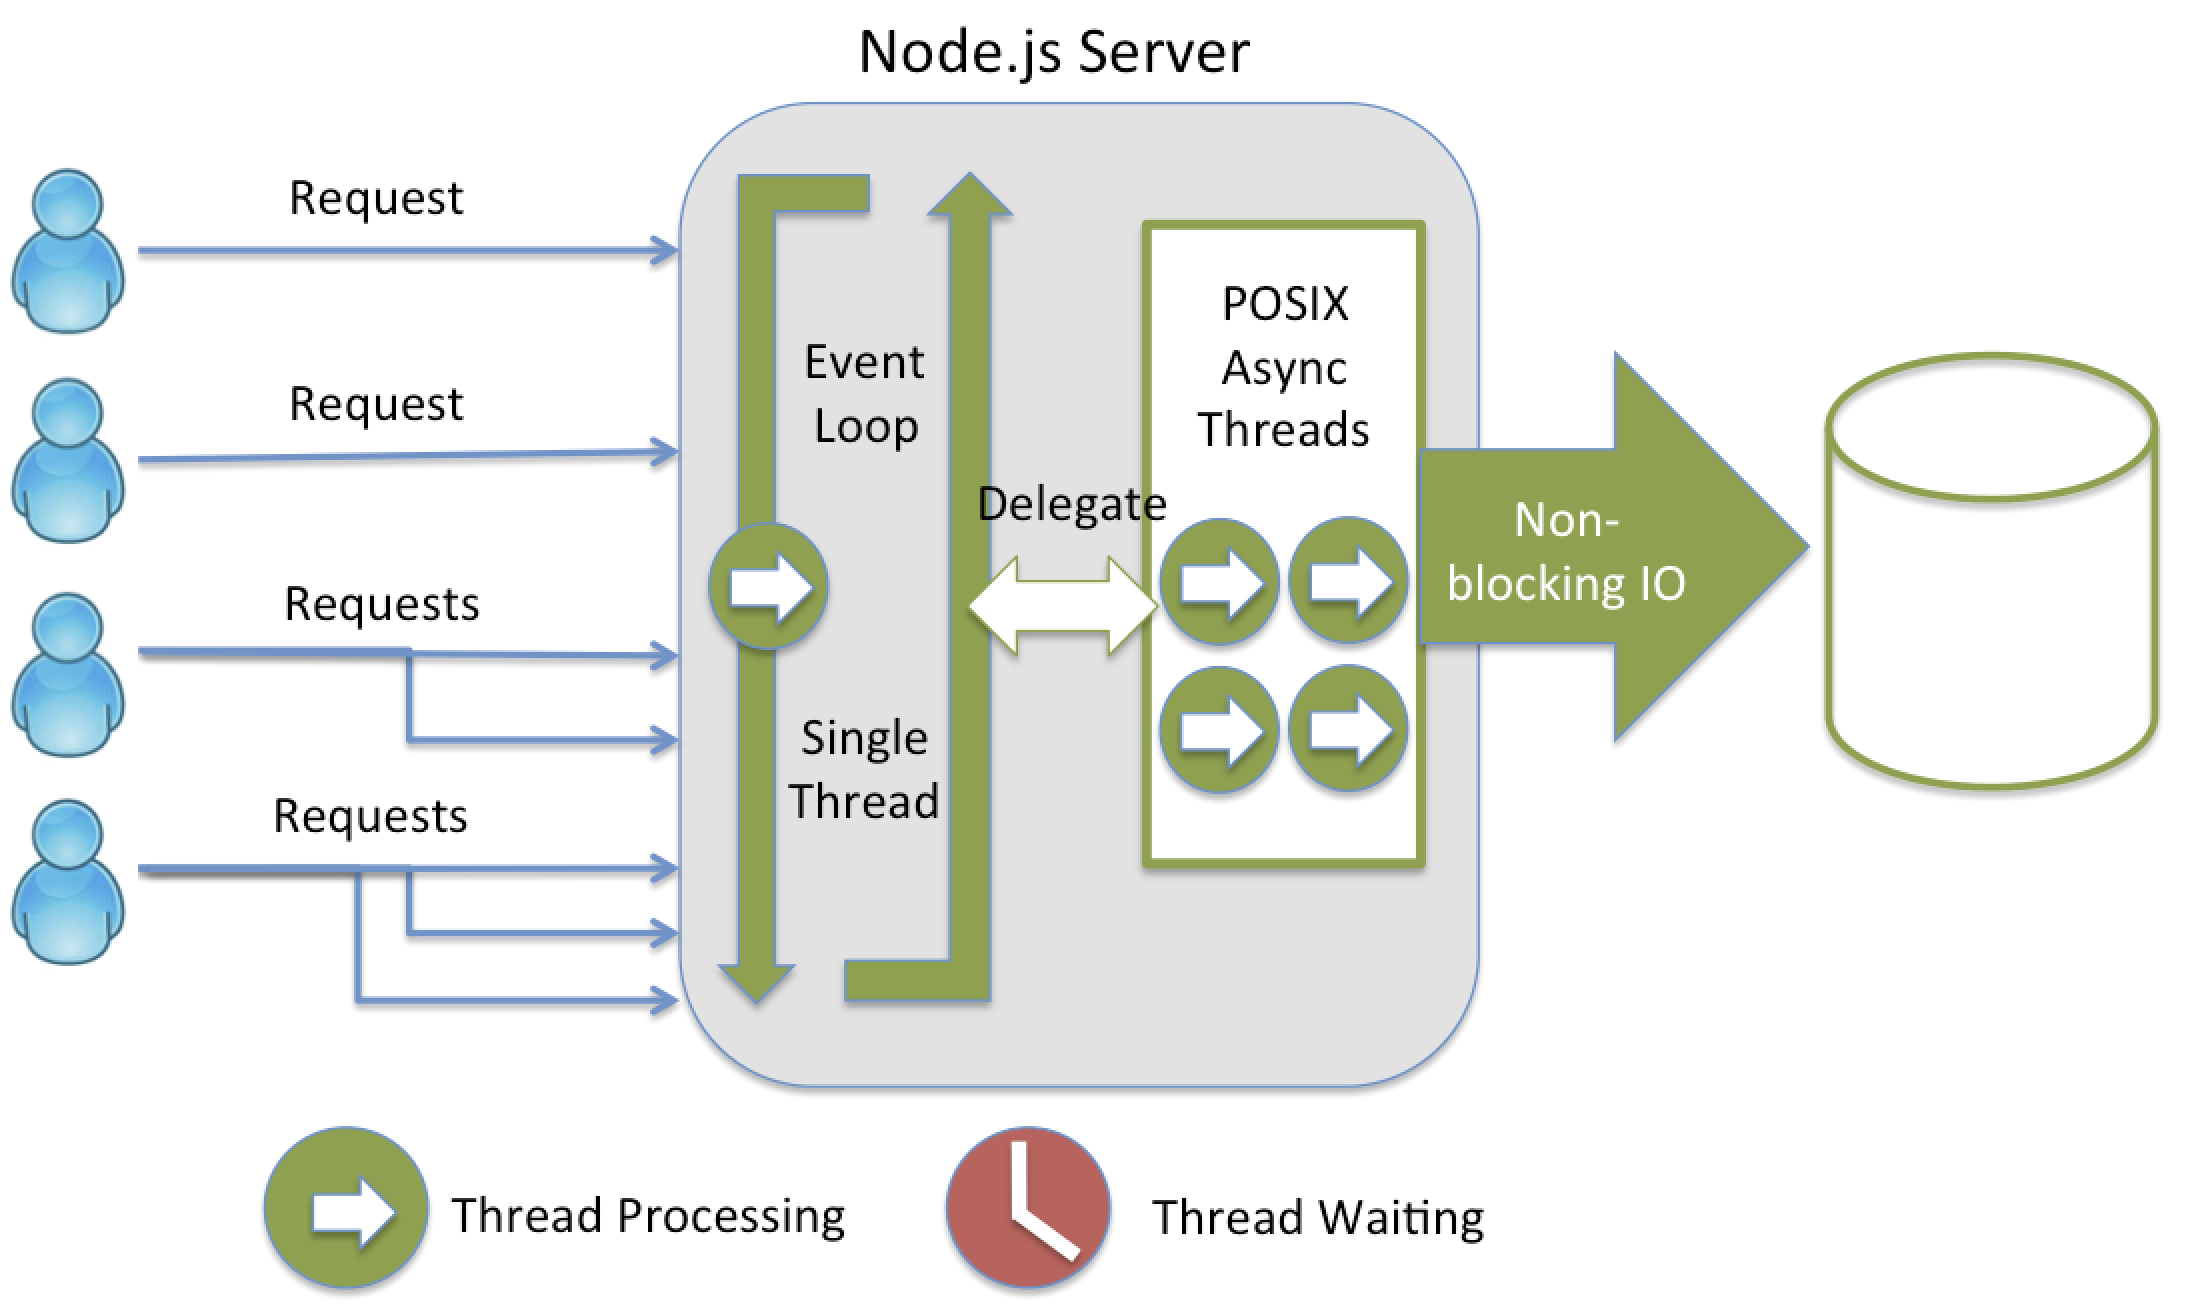
\includegraphics[width=10cm, height = 5.5cm]{images/nodejs_nodethreading.png}
\caption{ Single Threaded / Non Blocking I/0 [Nodejs 1.1]}
\end{figure}
 
 
Der große Vorteil hierbei ist, dass der Hauptthread trotz der blockierenden Ein- und Aus\-gabeoperationen nicht anhält, und weitere Anfragen bearbeiten kann. (Non Blocking I/O - Prinzip) 
\newline
